\documentclass[12pt]{article}

\usepackage{times}
\usepackage{amsmath, amssymb, multicol, graphicx}%pupr_paper,
\usepackage{listing}
\usepackage{verbatim}
\usepackage{booktabs}
\usepackage{float}
\usepackage[parfill]{parskip}
\usepackage{array}
\usepackage{caption}
%\lstset{language=C++}
\usepackage[colorlinks = true, linkcolor = blue]{hyperref}

\setlength{\textwidth}{6.5in} \setlength{\textheight}{8.5in} \topmargin -0.3in \setlength{\rightmargin}{0.0in}
\setlength{\leftmargin}{.0in} \setlength{\oddsidemargin}{.0in} \labelwidth=1.2in \labelsep=0.1in
\parsep=0in
\parindent=0in
%\pagestyle{empty}
\setcounter{secnumdepth}{3}
\floatstyle{boxed}
\restylefloat{figure}

\begin{document}
%\clearpage\pagenumbering{roman}
\begin{titlepage}
%\clearpage\pagenumbering{roman}
%\maketitle
 \centering
 Polytechnic University of Puerto Rico\\
 Hato Rey, Puerto Rico\\
 Department of Electrical and Computer Engineering and Computer Sciences\\
    \vspace*{15\baselineskip}
    \large
    \bfseries
    Software Project Management Plans  \\
    AIIPS Smart EyeSight\\
    Version 1.0\\[3\baselineskip]
    \normalfont
     \vfill
    Emanuel Rivera Castro 53502 \\
    Yanilette Lopez Duprey 53990\\
    Joaquin Pockels Balaguer 54012\\[2\baselineskip]

    \textbf{\today} \\
    COE 5002, FA-12\\
    Prof. Luis Ortiz Ortiz\\[2\baselineskip]
\end{titlepage}

\clearpage\pagenumbering{roman}
\setcounter{page}{2}
\begin{table}[H]\centering
\begin{tabular}{|>{\centering\arraybackslash}m{3cm}|>{\centering\arraybackslash}m{3cm}|
>{\centering\arraybackslash}m{3cm}|>{\centering\arraybackslash}m{3cm}|}
  \hline
  % after \\: \hline or \cline{col1-col2} \cline{col3-col4} ...
  Date & Version & Description & Author \\
   \hline
   9/26/2012 & 1.0 & First Draft & Emanuel Rivera \\
   \hline
\end{tabular}
\caption[]{Revision Table}
\end{table}
\pagebreak
\tableofcontents
\pagebreak
\listoftables
\pagebreak
\listoffigures
\clearpage\pagenumbering{arabic}

\section{Introduction}
 The purpose of this document, named Software Project Management Plan, is to establish in a clear form, the details and specifications of how this Project would be administrated. This document is going to facilitate the organization of the project, and it would guarantee that all the requirements are being fulfilled for the completion of the product.  This documents discuss the following topics:
\begin{itemize}
  \item Evolution of the SPMP
  \item Project Organization
  \item Managerial Process
  \item Technical Process
  \item Work Packages, Schedule and Budget
\end{itemize}
The SPMP is directed to:
\begin{enumerate}
  \item Clients - DARPA and Prof. Arturo Geigel
  \item Users - United States Armed Forces
  \item Developers - AIIP/S and people responsible for maintenance and making updates to the system.
\end{enumerate}

\subsection{Project Overview}
  The project is part of a proposal to Defense Advanced Research Projects Agency (DARPA). This proposal wants to decentralize control of unmanned vehicles, and allows multiple operators to operate a single vehicle or a formation of vehicles. This provides redundancy in the decision process and optimize the course of action to be followed. The main focus is the image segmentation and processing part. The images will be classify using a Probabilistic Neural Network (PNN) depending on the following features:
  \begin{itemize}
    \item Shape
    \item Color
    \item Location
    \item Normalized Area
    \item Texture
  \end{itemize}

\subsection{Project Deliverables}
This subsection list all the items to be delivered to the customer, the delivery dates, delivery locations, and quantities to satisfy the terms of the project.
\begin{itemize}
  \item IEEE 1058 Software Project Management Plan\\
            Due Date: October 31 2012 \\
            Quantity: 1\\
            Localization: L-310
  \item IEEE 830 Software Requirements Specification\\
            Due Date: October 31 2012\\
            Quantity: 1\\
            Localization: L-310
  \item IEEE 829 Software Test Document \\
            Due Date: October 31 2012\\
            Quantity: 1\\
            Localization: L-310

  \item IEEE 1016 Software Design Description\\
            Due Date: October 31 2012\\
            Quantity: 1\\
            Localization: L-310

  \item Image AIIPS Smart EyeSight\\
            Due Date:\\
            Quantity: 1\\
            Localization: L-310
\end{itemize}

\subsection{Evolution of the SPMP}
This subsection specify the plans for producing both scheduled and unscheduled updates, methods of disseminating the updates and to control subsequent changes to the SPMP.
\subsubsection{Updating the SPMP}
Any member would have all the right to present a motion to express his point of view.  If the point of view is valid and is seconded by the two other members, the document would be updated. Each time a member finish a section he/she will give it to the other members for review.

\subsubsection{Document Version}
The final version of the document will have the number 2.000. A change in the tenth position means that a new section was added, a change in the hundredth position means that a new subsection was added and a change in the thousandth position means that some subsection was modified.

\subsubsection{Tools}
Our main tool for updating this document is Github. Github is a repository where any member of the group can make changes without completely overwriting each other updates. As a second option, in case we experience any problems with Github, we will use dropbox to update this document.

\subsection{Reference Material}
This subsection provide a complete list of all the documents and other sources of information referenced in this document. Each document will be at least identified by title, author and date.

\subsubsection{IEEE Documents}
The following documents define the standards for the documentation of the AIPPS Smart EyeSight:
\begin{itemize}
  \item IEEE Std 1058.1-1987  Software Project Management Plan\\
				Author: The Software Engineering Technical Committee of the Computer Society of the IEEE\\
                Date: Approved December 10, 1987\\
				PDF: ISBN 0-7381-0409-4, SS12138

  \item IEEE Std 829-1998  Software Test Documentation\\
				Author: The Software Engineering Technical Committee of the Computer Society of the IEEE\\
                Date: Approved 16 September 1998
				PDF:ISBN 0-7381-1444-8 SS94687

  \item IEEE Std 830-1998 Software Requirement Specification \\
				Author: The Software Engineering Technical Committee of the Computer Society of the IEEE \\
                Date: Approved 25 June 1998\\
				PDF: ISBN 0-7381-0332-2

  \item IEEE Std 1016-1998 Software Design Description\\
				Author: The Software Engineering Technical Committee of the Computer Society of the IEEE\\
                Date: Approved 23 September 1998\\
				PDF: ISBN 0-7381-1456-1 SS94688	
\end{itemize}

\subsubsection{Papers}
The following research papers are necessary to develop AIIPS Smart EyeSight:
\begin{itemize}
  \item Region-Based Image Retrieval Using Probabilistic Feature Relevance Learning\\
        Author: ByoungChul Ko, Jing Peng and Hyeran Byun
  \item Probabilistic Neural Networks Supporting Multi-Class Relevance Feedback in Region-based Image Retrieval\\
        Author: ByoungChul Ko and Hyeran Byun\\
        Date: 2002
  \item FRIP: A Region-Based Image Retrieval Tool Using Automatic Image Segmentation and Stepwise Boolean AND Matching\\
        Author: ByoungChul Ko and Hyeran Byun\\
        Date: 2005
  \item A General Method for Unsupervised Segmentation of Images Using a Multiscale Approach\\
        Author: Alvin H. Kam and William J. Fitzgerald\\
        Date: 2000
\end{itemize}

\subsubsection{Books}
The following books are necessary to develop AIIPS Smart EyeSight:
\begin{itemize}
  \item Image Processing in C Second Edition\\
        Author: Dwayne Phillips
        Date: 2000
\end{itemize}

\subsection{Definitions and Acronyms}
This subsection shall define, or provide references to the definition of all terms and acronyms required to properly interpreted the SPMP.
\begin{table}[H]\centering
\begin{tabular}{|>{\centering\arraybackslash}m{7cm}|>{\centering\arraybackslash}m{7cm}|}
  \hline
  % after \\: \hline or \cline{col1-col2} \cline{col3-col4} ...
  Term & Definition \\
   \hline
   The Company & AIIPS \\
   \hline
   Software & Image Segmentation/Processing working code\\
   \hline
   Proposal & DARPA Proposal\\
   \hline
\end{tabular}
\caption{Definitions}
\end{table}

\begin{table}[H]\centering
\begin{tabular}{|>{\centering\arraybackslash}m{7cm}|>{\centering\arraybackslash}m{7cm}|}
  \hline
  % after \\: \hline or \cline{col1-col2} \cline{col3-col4} ...
  Term & Acronym \\
   \hline
   AIIPS & Artificial Intelligence and Image Processing/Segmentation   \\
    \hline
    PNN & Probabilistic Neural Network \\
    \hline
  Defense Advanced Research Projects Agency  & DARPA \\
   \hline
  Software Requirements Specification & SRS \\
   \hline
    Software Project Management Plan & SPMP \\
   \hline
     Software Test Document & STD \\
   \hline
     Software Design Description & SDD \\
     \hline
     Institute of Electrical and Electronics Engineers & IEEE\\
   \hline
\end{tabular}
\caption{Acronyms}
\end{table}

\section{Project Organization}
This section is divided in the following subsections:
\begin{itemize}
  \item Process Model
  \item Organizational Structure
  \item Organizational Boundaries and Interfaces
  \item Project Responsibilities
\end{itemize}

\subsection{Process Model}
The organization for the development of the software's documents (SRS, STD, SDD, SPMP and Smart EyeSight Code) will be paralleled, lineal and incremental. Each member will have a document assigned, this way the documents can be completed by the due date the client specify.\\\\
The following figure (\ref{org_struct}) shows the process model of the project.

\begin{figure}[H]\centering
  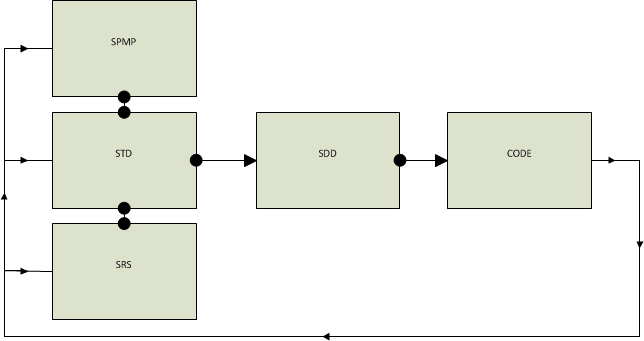
\includegraphics[width=6.0in]{block_diagram_Org_Struct}\\
  \caption{Block Diagram of the Process Model}\label{org_struct}
  \end{figure}

\subsection{Organizational Structure}
AIIPS is compose of 3 members, each with a main position in the team, primary and secondary tasks. The following figure (\ref{org_diagram}) shows the positions within the organization, the primary and Secondary Tasks of each member:

\begin{figure}[H]\centering
  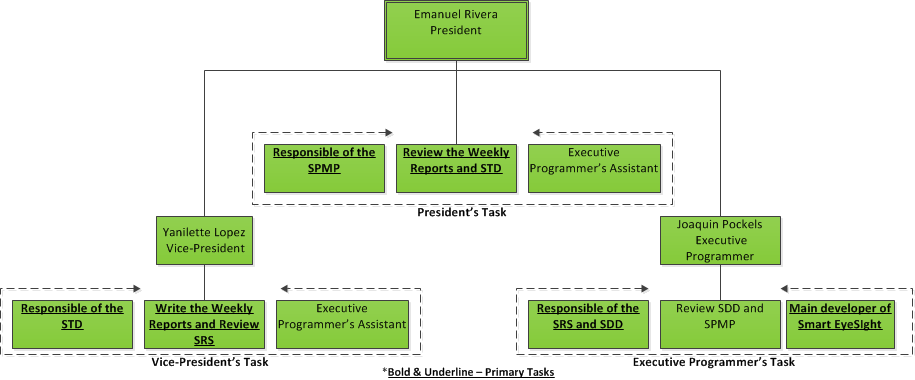
\includegraphics[width=6.0in]{org_diagram}\\
  \caption{Organizational Diagram}\label{org_diagram}
  \end{figure}

Decisions within the Company are handled through voting. The changes must be discussed by the group, after which a debate will take place to find the advantages and disadvantages. Finally, the group will vote and majority decided whether the change will take place. Each meeting will be documented in the weekly report.\\\\
Communication between group members will consist of phone calls, text messages and meetings. Generally, meetings take place every Wednesday at 1:30pm with additional meetings taking place during whenever the group decides is necessary.

\subsection{Organizational Boundaries and Interfaces}
As section 1 of this documents says the main purpose/objective in the project is to implement the image segmentation/processing of the DARPA proposal. For the purpose of testing 150 images were selected to verify the effectiveness of Smart EyeSight (Please refer to the STD Document for more information). In a real situation Smart EyeSight will be receiving images from an external agent, robot and/or UAV. Then the images will be segmented and classify and the classification will be send to the external agent. Other companies/organizations will take care of the other components of this proposal.\\\\
Figure \ref{boundaries} shows the relevant parts for this project of the DARPA proposal. We don't care who or how the other agents do their work, our only concern is to have images as input to our Software.

\begin{figure}[H]\centering
  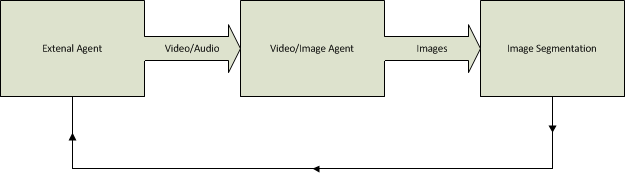
\includegraphics[width=6.0in]{boundaries}\\
  \caption{Block Diagram of the Boundaries of our Project}\label{boundaries}
  \end{figure}

\subsection{Project Responsibilities}
It is important to note that there will be at least one manager per document. The manager(s) of the document will be listed with the documents type also indicating the other member(s) that were assigned to work under that document.Tables \ref{RespMem}-\ref{RespSPMP} shows the responsibilities of each member.

\begin{table}[H]\centering
\begin{tabular}{|>{\centering\arraybackslash}m{5cm}|>{\centering\arraybackslash}m{5cm}|>{\centering\arraybackslash}m{5cm}|}
  \hline
  % after \\: \hline or \cline{col1-col2} \cline{col3-col4} ...
  Document & Project Manager(s) & Assistant Member(s) \\
   \hline
   AIIPS SRS & Joaquin Pockels & Emanuel Rivera, Yanilette Lopez \\
   \hline
   AIIPS SDD & Joaquin Pockels & Emanuel Rivera, Yanilette Lopez\\
   \hline
   AIIPS STD & Yanilette Lopez & Emanuel Rivera, Joaquin Lopez  \\
   \hline
   AIIPS SPMP & Emanuel Rivera & Joaquin Lopez, Yanilette Lopez \\
   \hline
   AIIPS Software & Joaquin Pockels & Emanuel Rivera, Yanilette Lopez \\
   \hline
\end{tabular}
\caption{Main Responsibilities for each member}
\label{RespMem}
\end{table}

\begin{table}[H]\centering
\begin{tabular}{|>{\centering\arraybackslash}m{5cm}|>{\centering\arraybackslash}m{5cm}|>{\centering\arraybackslash}m{5cm}|}
  \hline
  \multicolumn{3}{|c|}{SRS} \\
  \hline
  % after \\: \hline or \cline{col1-col2} \cline{col3-col4} ...
  Title & Section(s) & Member(s) \\
   \hline
    &  &  \\
   \hline
\end{tabular}
\caption{Shows who works in each section of the SRS}
\label{RespSRS}
\end{table}

\begin{table}[H]\centering
\begin{tabular}{|>{\centering\arraybackslash}m{5cm}|>{\centering\arraybackslash}m{5cm}|>{\centering\arraybackslash}m{5cm}|}
  \hline
  \multicolumn{3}{|c|}{SDD} \\
  \hline
  % after \\: \hline or \cline{col1-col2} \cline{col3-col4} ...
  Title & Section(s) & Member(s) \\
   \hline
    Introduction & 1 & Emanuel Rivera \\
   \hline
\end{tabular}
\caption{Shows who works in each section of the SDD}
\label{RespSDD}
\end{table}

\begin{table}[H]\centering
\begin{tabular}{|>{\centering\arraybackslash}m{5cm}|>{\centering\arraybackslash}m{5cm}|>{\centering\arraybackslash}m{5cm}|}
  \hline
  \multicolumn{3}{|c|}{STD} \\
  \hline
  % after \\: \hline or \cline{col1-col2} \cline{col3-col4} ...
  Title & Section(s) & Member(s) \\
   \hline
    &  &  \\
   \hline
\end{tabular}
\caption{Shows who works in each section of the STD}
\label{RespSTD}
\end{table}

\begin{table}[H]\centering
\begin{tabular}{|>{\centering\arraybackslash}m{5cm}|>{\centering\arraybackslash}m{5cm}|>{\centering\arraybackslash}m{5cm}|}
  \hline
  \multicolumn{3}{|c|}{SPMP} \\
  \hline
  % after \\: \hline or \cline{col1-col2} \cline{col3-col4} ...
  Title & Section(s) & Member(s) \\
   \hline
   Introduction, Project Organization, Managerial Process, Technical Process, Work Packages, Schedule, and Budget & 1-5  & Emanuel Rivera \\
   \hline
\end{tabular}
\caption{Shows who works in each section of the SPMP}
\label{RespSPMP}
\end{table}

\section{Managerial Processes}
This section is divided in the following subsections:
\begin{itemize}
  \item Management objectives and priorities
  \item Project assumptions, dependencies and constraints
  \item Risk management techniques
  \item Monitoring and controlling mechanisms to be used
  \item Staffing Plan
\end{itemize}

\subsection{Management Objectives and Priorities}
This section contains the philosophy, goals and priorities on management activities for the project. Also it specify the format used for reporting and the expected frequency of reports, priorities of requirements, schedule and budget.

\subsubsection{Philosophy}
The philosophy adopted for the management of activities is: divide and conquer. The group will usually meet; either physically or via other means of communication, such as, internet conference calls using Skype or phone calls. Afterwards, the activity is discussed by the members and decomposed into essential parts or tasks required for the activity completion which are then assigned to the corresponding member.

\subsubsection{Goals}
The goals are simply to be able to fulfill the objectives of this stage of the Proposal and writing each document as fast as possible so we can have feedback from our client, review, audit and proceed to the next activity.

\subsubsection{Priorities}
The priorities on an activity may vary on the difficulty and/or length of the activity. The order established for the main activity priorities are the following:

\begin{enumerate}
  \item Documenting the plan (SPMP) and the requirements (SRS) of the Project.
  \item Documenting the design (SDD) and testing methods (STD) of the Project.
  \item Work on AIIPS Smart EyeSight. 
  \item Meet with our client for feedback.
\end{enumerate}

\subsubsection{Project Budget Priorities}
The priority on the project budget allocation is the following:
\begin{itemize}
  \item Computers for the project staff
  \item Required hardware and software for the project’s completion. (Refer to section 4.1 for list of software and hardware)
  \item Papers and books necessary for a better understanding of the process/steps to complete this Project. (Refer to sections 1.4.2 and 1.4.3 for list of papers and books)
\end{itemize}

\subsubsection{Risk Management Procedures}
In the event that a risk or problematic situation occurs during the development of the project, an emergency staff meeting will take place in order to address the problem or situation. On these meeting it’s imperative to hear each of the staff member’s opinion and possible solutions on the matter. Afterwards the project staff will proceed to make a democratic vote election to determinate the course of action to be taken based on the proposed or accepted solutions to the given risk or problem.

\subsubsection{Software Acquisition Statement Management}
The proper format to deliver a statement which states the intention of acquiring, modifying or using existing software should follow the following procedure:

\begin{itemize}
  \item	Mention the Software in question during a staff meeting.
  \item State the reasons why the existing software is needed.
  \item Mention and justify the amount of software licenses needed
  \item Afterwards the staff in democratic vote will decide to acquire the software or not.
\end{itemize}

\subsection{Assumptions, Dependencies and Constraints}
This section will contain the following information:

 \begin{itemize}
   \item The necessary assumptions on which the project is based.
   \item External events the project is dependent upon in order to be completed.
   \item Constraints on which the project will be conducted.
 \end{itemize}

\subsubsection{Assumptions}
The assumptions for this project are the following:

\begin{enumerate}
  \item AIIPS will not design the external agent that will capture the video and audio. The client needs the agent that will capture the video and audio.
  \item AIIPS will not design the communication protocol to send the video. The client needs to have the communication protocol to send the video.
  \item AIIPS will not design the process/algorithm to "change" the video into frames/images. The client need to have the process/algorithm to take the video and divide it in frames/images.
\end{enumerate}
\subsubsection{Dependencies}
Most of the dependencies of external events the project will be dependent upon will be due the completion of the project documentations. For example SDD and STD documents will be dependent on the completion of the SRS and SPMP documentations in order for their completion to be successful. Other dependencies would be the feedback from our client that may change/alter the code and/or documents.
\subsubsection{Constraints}
The following are the constraints of the project:
\begin{enumerate}
  \item Smart EyeSight have a time constraint of 3 months for documenting the software and 6 months to have a working code.
  \item Project documents must comply with IEEE software documentation format
  \item All the requirements mentioned in the SRS.
\end{enumerate}

\subsection{Risk Management}
This subsection identify and assess the risk factors associated with the project. It prescribe mechanisms for tracking the various risk factors and implementing contingency plans.

\subsubsection{Risk regarding contract}
  Examples would be not complying with the established deadline by the costumer. Another example would be violations of the contract terms from either end of the contract. These are the most common situations that may occur during project development.
\subsubsection{Risk’s regarding technology related on the project}
      An example would be damage received to project data resulting in it’s loss. Other situations that could occur are damage or theft of computer equipment or other materials.
\subsubsection{Risk’s regarding size and complexity of the product}
      An example of these risks would be that requirements and constraints of the project may require strong attention to detail and extensive documentation that may require more time that the established deadline. Another example could be disagreement on the design approach to solve a particular problem regarding the project’s development which may result on delaying progress on the project’s development.
\subsubsection{Risks regarding personnel acquisition and retention}
      Examples of these risks would be that a member may not have the required skill and expertise in order to perform assigned tasks which would hinder greatly the project’s development. Another example would be that a project staff member doesn’t complete the assigned task or that the completed task does not meet the expected standards. Another possible example would be the inconsistency of a project member to show up on meetings or having lack of communication with other project staff members resulting in a hindrance to the project’s development for not being in par with the progress of the project’s development.
\subsubsection{Risks regarding consumer acceptance of the product}
      Examples would be the customer may not express the desired resulting product correctly and mid development forces the staff member to redo most of the currently developed product on the project. Another example would be additional requests from the customer that may require drastic changes on the currently developed product.  Finally a risk example would be that the final product doesn’t comply with the requirements and constraints given by the client resulting in customer’s dissatisfaction, termination of the contract, revenue loss, loss of the company’s reputation, company bankruptcy and other undesired situations.

\subsection{Monitoring and Controlling Mechanisms} 
Process to request a change in the document:
\begin{enumerate}
  \item Client, Users and/or Developer(AIIPS member) request a change in a document after reviewing it.
  \item The member assigned to that particular document makes the changes necessary to comply with the change request using WinEdt 7 or Emacs. The responsibility to makes the changes can be given to another member if there is a valid reason. (sickness, minor changes, education, family)
  \item The member assigned to that particular document uploads the document to GitHub and DropBox, this keeps each member informed about the documentation progress.
\end{enumerate}
For more information about each member responsibilities go to section 2.2 and 2.4

\subsection{Staffing Plan}
The Project can be developed with a small group consisting of three (3) members. They, however, have to meet the following requirements:
\begin{enumerate}
  \item Have Experience with C.
  \item Start working in August 13, 2012.
  \item Work until February 2013.
  \item Have time to attend meetings.
  \item Have a Bachelor degree on computer science or Computer Engineering.
  \item Work on flexible schedules.
  \item Have knowledge or experience with PNN.
  \item Follow instructions.
  \item Work in a team.
  \item Basic knowledge of IEEE standard software documentation.
\end{enumerate}

\section{Technical Process}
This section specify the technical methods, tools, and techniques to be used on the project. This section is divided in the following subsections:
\begin{itemize}
  \item Methods, Tools, and Techniques
  \item Software Documentation
  \item Project Support Functions
\end{itemize}

\subsection{Methods, Tools, and Techniques}
In order to bring this project together, extensive resources were needed. This includes, but is not limited to these tools:

\begin{itemize}
  \item Microsoft Office Projects 2010
  \item Linux Ubuntu 12.04.1
  \item Microsoft Windows 07
  \item Microsoft Office Visio 2010
  \item ASUS A53S Series
  \item ASUS G53SX-XT1
  \item ASUS Notebook G60 Series
  \item Visual Studios 2010
  \item GCC, the GNU Compiler Collection
  \item Emacs, Winedt 7, Miktex 2.9 (Latex)
\end{itemize}

For the Methods and Techniques to be used please see section 2.1 and 2.2

\subsection{Software Documentation}
The Process of documentation is based on the standard documents of The Institute of Electrical and Electronics Engineers (IEEE). Here is a description of the documents that we use on this project.

\subsubsection{Software Project Management Plan}
The software project management plan is the controlling document for managing a software project; it defines the technical and managerial processes necessary to satisfy the project requirements.

\subsubsection{Software Requirements Specification}
The software requirements specification is an important part of the requirements process of the software life cycle and is used in design, implementation, project monitoring, verification and validation. It gives a complete description of the behavior of the system to be developed.

\subsubsection{Software Test Document}
The standardized test document can facilitate communication by providing a common frame of reference. Serves as a completeness checklist for the associated testing process; can also provide a baseline for the evaluation of the current test practices.

\subsubsection{Software Design Description}
The software design description is a representation of a software system that is used as a medium for communicating software design information. A representation of a software system is created to facilitate analysis, planning, implementation, and decision making.

\subsection{Project Support Functions}
Updates for Smart EyeSight will be periodically every month for the first year after launch. After the first year updates will be make every four (4) months and after the second year, every six (6) months. Only a client request for an update can change the establish time. After each update AIIPS will test the software and write a detail report of the changes to Smart EyeSight. Then the software, with the updates, will be implemented back in the system. The following figure (\ref{support} shows the procedure to deliver an update.

\begin{figure}[H]\centering
  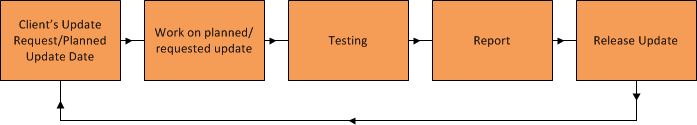
\includegraphics[width=6.0in]{project_support}\\
  \caption{Block Diagram of the Process to maintain and deliver updates to Smart EyeSight}\label{support}
  \end{figure}

\section{Work Packages, Schedule, and Budget}
This section specify the work packages, identify the dependency relationships among them, state the resource requirements, provide allocation of budget and resources to work packages, and establish a project schedule. This section is divided in the following subsections:
\begin{itemize}
  \item Work Packages
  \item Dependencies
  \item Resource Requirements
  \item Budget and Resource Allocation
  \item Schedule
\end{itemize}

\subsection{Work Packages}
In order to complete the project agreement, the client will receive four (4) documents described in the Software Documentation section (4.2) and in the following 3-4 months a working code of Smart EyeSight.

\subsection{Dependencies}
The dependencies for these work packages are detailed in Figure \ref{dependencies}.

\begin{figure}[H]\centering
  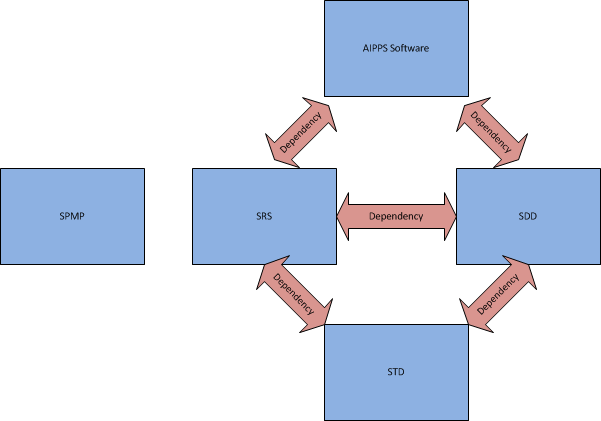
\includegraphics[width=4.372in]{dependencies}\\
  \caption{Block Diagram of the Dependencies of our Project}\label{dependencies}
  \end{figure}

\subsection{Resource Requirements}
Please see section 4.1 for the Resources/Tools needed for the completion of this project.

\subsection{Budget and Resource Allocation}
\begin{table}[H]\centering
\begin{tabular}{|>{\centering\arraybackslash}m{3.5cm}|>{\centering\arraybackslash}m{3.5cm}|>{\centering\arraybackslash}m{3.5cm}|>{\centering\arraybackslash}m{3.5cm}|}
  \hline
  % after \\: \hline or \cline{col1-col2} \cline{col3-col4} ...
  Items & Quantity & Amount & Total\\
   \hline
   Laptops & 3 & \$750 + \$900 + \$ 1200  & \$2850\\
   \hline
   Gasoline & 2 & \$250 & \$500\\
   \hline
   Office 2010 Professional & 3 & \$408.99 & \$1226.97 \\
   \hline
    Office Project 2010 & 1 & \$499.80 & \$499.80 \\
   \hline
   TOTAL & & &\$5076.77\\
   \hline
\end{tabular}
\caption{Shows the cost of Resources for this Project}
\label{resources}
\end{table}

\begin{table}[H]\centering
\begin{tabular}{|>{\centering\arraybackslash}m{3.5cm}|>{\centering\arraybackslash}m{3.5cm}|>{\centering\arraybackslash}m{3.5cm}|>{\centering\arraybackslash}m{3.5cm}|}
  \hline
  % after \\: \hline or \cline{col1-col2} \cline{col3-col4} ...
  Personnel  & Months & Amount(Per Month) & Total\\
   \hline
   Emanuel Rivera & 6 & \$2500  & \$15000\\
   \hline
   Joaquin Pockels & 6 & \$2000 & \$12000\\
   \hline
   Yanilette Lopez & 6 & \$2000 & \$12000 \\
   \hline
    TOTAL & & &\$39000\\
    \hline
\end{tabular}
\caption{Shows the cost of Personnel for this Project}
\label{personnel}
\end{table}

\begin{table}[H]\centering
\begin{tabular}{|>{\centering\arraybackslash}m{7.5cm}|>{\centering\arraybackslash}m{7.5cm}|}
  \hline
  % after \\: \hline or \cline{col1-col2} \cline{col3-col4} ...
  Resources  & Total\\
   \hline
   Materials/Tools & \$5076.77\\
   \hline
   Human Resources & \$39000\\
   \hline
    TOTAL & \$44076.77\\
   \hline
\end{tabular}
\caption{Shows the total cost for this Project}
\label{total}
\end{table}
\subsection{Schedule}

\end{document}
